% MH1812 — Chapter 3: Functions (0->100 ground-up)
\chapter[Functions]{Functions: Injections, Surjections, Bijections and Cardinality}
\label{ch:functions}

\begin{quote}
\emph{``A function is a machine that turns inputs into outputs.''} --- yet not every machine is reversible, and not every output is hit. Injectivity, surjectivity and size make this precise.
\end{quote}

\noindent\fbox{\parbox{\dimexpr\linewidth-2\fboxsep-2\fboxrule}{%
\textbf{From zero: arrows between bags.} Picture two bags of dots (domain, codomain) with arrows $a\mapsto f(a)$. We classify when arrows never collide (injective), cover everything (surjective), or both (bijective), then use bijections to compare sizes --- even for infinite sets.}}
\vspace{0.4em}

\section*{Learning Outcomes}
After this chapter you will be able to:
\begin{enumerate}[label=(L\arabic*)]
    \item define function, domain, codomain, image, preimage, composition;
    \item test injectivity, surjectivity, bijectivity with arrow and algebraic criteria;
    \item invert bijective functions and reason about composition;
    \item compare cardinalities via bijections and prove countability results;
    \item explain why $|\mathbb{N}|=|\mathbb{Z}|=|\mathbb{Q}|<|\mathbb{R}|$ (diagonal).
\end{enumerate}

% ============================================================
\section{Functions as Deterministic Arrows}
\label{sec:functions-def}
A \emph{function} $f:A\to B$ assigns to each $a\in A$ exactly one $b=f(a)\in B$. $A$ is the \emph{domain}, $B$ the \emph{codomain}. The \emph{image} (range) $f(A)=\{f(a):a\in A\}\subseteq B$ may be smaller than $B$. The \emph{preimage} $f^{-1}(T)=\{a:f(a)\in T\}$ lifts subsets backwards.

Think of a lookup table: one output per input, never zero or two. Vertical-line test is the picture: every $a$ has exactly one outgoing arrow.

\begin{figure}[h]\centering
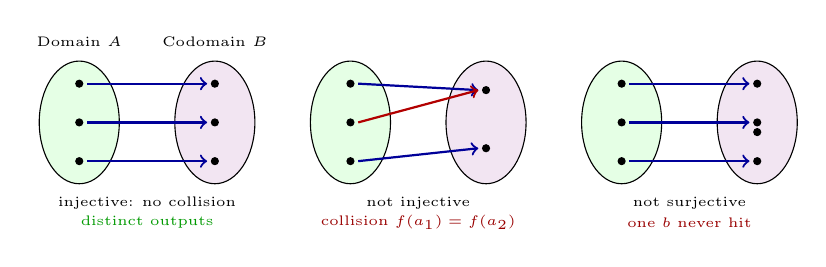
\begin{tikzpicture}[scale=0.82,every node/.style={font=\scriptsize}]
% injective vs non-injective vs surjective
\begin{scope}
\draw[rounded corners=3pt,fill=green!10] (0,0) ellipse (0.62 and 0.95);
\draw[rounded corners=3pt,fill=violet!10] (2.1,0) ellipse (0.62 and 0.95);
\node[font=\tiny] at (0,1.25) {Domain $A$}; \node[font=\tiny] at (2.1,1.25) {Codomain $B$};
\foreach \y/\yy in {0.6/0.6,0.0/0.0,-0.6/-0.6} {\fill (0,\y) circle (1.8pt); \fill (2.1,\yy) circle (1.8pt); \draw[->,thick,blue!60!black] (0.12,\y)--(1.98,\yy);}
\node[font=\tiny,fill=white,inner sep=1pt] at (1.05,-1.25) {injective: no collision};
\node[font=\tiny,green!60!black] at (1.05,-1.55) {\checkmark distinct outputs};
\end{scope}
\begin{scope}[xshift=4.2cm]
\draw[rounded corners=3pt,fill=green!10] (0,0) ellipse (0.62 and 0.95);
\draw[rounded corners=3pt,fill=violet!10] (2.1,0) ellipse (0.62 and 0.95);
\foreach \y in {0.6,0.0,-0.6} \fill (0,\y) circle (1.8pt);
\foreach \y in {0.5,-0.4} \fill (2.1,\y) circle (1.8pt);
\draw[->,thick,blue!60!black] (0.12,0.6)--(1.98,0.5);
\draw[->,thick,red!70!black] (0.12,0.0)--(1.98,0.5);
\draw[->,thick,blue!60!black] (0.12,-0.6)--(1.98,-0.4);
\node[font=\tiny,fill=white,inner sep=1pt] at (1.05,-1.25) {not injective};
\node[font=\tiny,red!60!black] at (1.05,-1.55) {collision $f(a_1)=f(a_2)$};
\end{scope}
\begin{scope}[xshift=8.4cm]
\draw[rounded corners=3pt,fill=green!10] (0,0) ellipse (0.62 and 0.95);
\draw[rounded corners=3pt,fill=violet!10] (2.1,0) ellipse (0.62 and 0.95);
\foreach \y in {0.6,0.0,-0.6} \fill (0,\y) circle (1.8pt);
\foreach \y in {0.6,0.0,-0.6, -0.15} \fill (2.1,\y) circle (1.8pt);
\draw[->,thick,blue!60!black] (0.12,0.6)--(1.98,0.6);
\draw[->,thick,blue!60!black] (0.12,0.0)--(1.98,0.0);
\draw[->,thick,blue!60!black] (0.12,-0.6)--(1.98,-0.6);
\node[font=\tiny,fill=white,inner sep=1pt] at (1.05,-1.25) {not surjective};
\node[font=\tiny,red!60!black] at (1.05,-1.55) {one $b$ never hit};
\end{scope}
\end{tikzpicture}
\caption{Arrow tests for injectivity and surjectivity. Bijective = both: perfect matching.}
\label{fig:function-types}
\end{figure}

\begin{definition}[Injective, surjective, bijective]
$f:A\to B$ is \emph{injective} (one-to-one) if $f(a_1)=f(a_2)\Rightarrow a_1=a_2$ (no two arrows share a target). \emph{Surjective} (onto) if $\forall b\in B\,\exists a\in A\,f(a)=b$ (every $b$ is hit). \emph{Bijective} if both.
\end{definition}

\begin{example}
$f:\mathbb{N}\to\mathbb{N},\,f(n)=2n$ is injective (if $2a=2b$ then $a=b$) but not surjective (odd numbers missed). $g:\mathbb{R}\to\mathbb{R},\,g(x)=x^3$ is bijective; $h:\mathbb{R}\to\mathbb{R},\,h(x)=x^2$ is neither.
\end{example}

Composition $(g\circ f)(a)=g(f(a))$ is associative; identity $\mathrm{id}_A(a)=a$ is bijective. If $f,g$ injective then $g\circ f$ injective; similarly for surjective/bijective.

\section{Inverses and Composition}
\label{sec:inverses}
$f:A\to B$ has an \emph{inverse} $f^{-1}:B\to A$ iff $f$ is bijective, with $f^{-1}(b)=$ the unique $a$ with $f(a)=b$. Then $f^{-1}\circ f=\mathrm{id}_A$ and $f\circ f^{-1}=\mathrm{id}_B$.

Test: to show $f$ bijective, exhibit an explicit inverse. For $f:\mathbb{Z}\to\mathbb{Z}$, $f(n)=n+1$ has $f^{-1}(m)=m-1$.

\begin{lemma}[Composition preserves type]
If $f:A\to B$ and $g:B\to C$ are bijections, so is $g\circ f$, with $(g\circ f)^{-1}=f^{-1}\circ g^{-1}$ (socks-and-shoes).
\end{lemma}

\begin{figure}[h]\centering
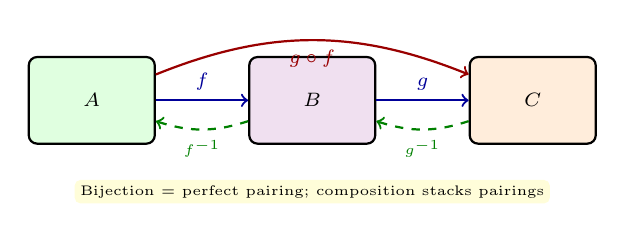
\begin{tikzpicture}[scale=0.80,every node/.style={font=\scriptsize}]
% Composition diagram
\node[draw,thick,rounded corners=3pt,fill=green!12,minimum width=1.6cm,minimum height=1.1cm] (A) at (0,0) {$A$};
\node[draw,thick,rounded corners=3pt,fill=violet!12,minimum width=1.6cm,minimum height=1.1cm] (B) at (3.5,0) {$B$};
\node[draw,thick,rounded corners=3pt,fill=orange!14,minimum width=1.6cm,minimum height=1.1cm] (C) at (7,0) {$C$};
\draw[->,thick,blue!60!black] (A)--(B) node[midway,above] {$f$};
\draw[->,thick,blue!60!black] (B)--(C) node[midway,above] {$g$};
\draw[->,thick,red!60!black,bend left=22] (A) to node[midway,below] {$g\circ f$} (C);
% inverse arrows dashed
\draw[->,thick,dashed,green!50!black] (B) to[bend left=18] node[midway,below,font=\tiny] {$f^{-1}$} (A);
\draw[->,thick,dashed,green!50!black] (C) to[bend left=18] node[midway,below,font=\tiny] {$g^{-1}$} (B);
\node[font=\tiny,fill=yellow!15,rounded corners=2pt,inner sep=2pt] at (3.5,-1.45) {Bijection $=$ perfect pairing; composition stacks pairings};
\end{tikzpicture}
\caption{Composition and inverses: bijective arrows pair elements one-to-one.}
\label{fig:composition-inverse}
\end{figure}

\begin{lstlisting}[language=Python]
# Checking injectivity/surjectivity by brute force on finite sets
def is_injective(f, A): 
    seen={}
    for a in A:
        b=f(a)
        if b in seen: return False, (seen[b], a, b)
        seen[b]=a
    return True, None

def is_surjective(f, A, B): return all(any(f(a)==b for a in A) for b in B)
print(is_injective(lambda x: 2*x, {0,1,2,3}))
print(is_surjective(lambda x: 2*x, {0,1,2,3}, {0,1,2,3,4,5,6}))
\end{lstlisting}

% ============================================================
\section{Cardinality: Comparing Sizes via Bijections}
\label{sec:cardinality}
We say $|A|=|B|$ iff a bijection $A\to B$ exists; $|A|\le|B|$ iff an injection $A\to B$ exists. For finite sets this matches counting; for infinite sets it surprises.

$|\mathbb{N}|=|\mathbb{Z}|$: enumerate $0,1,-1,2,-2,\dots$ gives bijection $f:\mathbb{N}\to\mathbb{Z}$.
$|\mathbb{N}|=|\mathbb{N}\times\mathbb{N}|$: Cantor pairing $(m,n)\mapsto 2^m3^n$ injection and diagonal enumeration bijection; $|\mathbb{Q}|=|\mathbb{N}|$ via reduced fractions grid traversal.

But $|\mathbb{R}|>|\mathbb{N}|$. Cantor's diagonal: assume listing $r_1,r_2,\dots$ of $(0,1)$ in decimal; build $d$ whose $i$th digit differs from $i$th digit of $r_i$; $d$ not in listing --- contradiction. Hence reals are \emph{uncountable}.

\begin{figure}[h]\centering
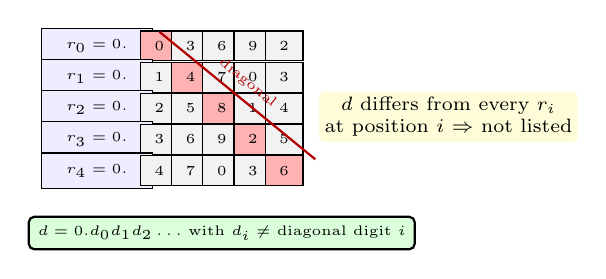
\begin{tikzpicture}[scale=0.72,every node/.style={font=\tiny}]
% Diagonal argument picture
\foreach \i in {0,...,4} {
  \node[draw,fill=blue!7,minimum width=1.4cm,minimum height=0.45cm] at (0,-\i*0.55) {$r_{\i}=0.$};
  \foreach \j in {0,...,4} {
    \pgfmathsetmacro{\x}{1.1 + \j*0.55}
    \pgfmathsetmacro{\col}{\i==\j ? "red!30" : "gray!10"}
    \node[draw,fill=\col,minimum width=0.48cm,minimum height=0.38cm] at (\x,-\i*0.55) {\pgfmathparse{int(mod(\i+\j*3,10))}\pgfmathresult};
  }
}
\draw[thick,red!70!black] (1.1,0.25)--(3.85,-2.0) node[midway,above,sloped,font=\tiny] {diagonal};
\node[draw,thick,fill=green!14,rounded corners=2pt,minimum width=4.5cm] at (2.2,-3.3) {$d=0.d_0d_1d_2\dots$ with $d_i\neq$ diagonal digit $i$};
\node[font=\scriptsize,fill=yellow!15,rounded corners=2pt,inner sep=2pt,align=center] at (6.2,-1.25) {$d$ differs from every $r_i$\\at position $i$ $\Rightarrow$ not listed};
\end{tikzpicture}
\caption{Cantor diagonal: the red diagonal builds a real $d$ absent from any enumeration, so $\mathbb{R}$ is uncountable.}
\label{fig:cantor-diagonal}
\end{figure}

\begin{theorem}[Cantor--Bernstein--Schroeder, stated]
If $|A|\le|B|$ and $|B|\le|A|$ then $|A|=|B|$.
\end{theorem}

\begin{remark}[Pigeonhole preview]
If $|A|>|B|$ no injection $A\to B$ exists (pigeonhole, Ch.~5). For finite $A$, $f:A\to A$ is injective iff surjective iff bijective.
\end{remark}


\begin{example}[Images and preimages]
For $f:\mathbb{R}\to\mathbb{R},\,f(x)=x^2$, $f(\{-2,2\})=\{4\}$, $f^{-1}(\{4\})=\{-2,2\}$, $f^{-1}(\{-1\})=\emptyset$. Images preserve unions; preimages preserve all Boolean operations.
\end{example}

\begin{theorem}[Preimage preserves Boolean structure]
For any $f:A\to B$ and $X,Y\subseteq B$, $f^{-1}(X\cup Y)=f^{-1}(X)\cup f^{-1}(Y)$, $f^{-1}(X\cap Y)=f^{-1}(X)\cap f^{-1}(Y)$, $f^{-1}(\bar X)=\overline{f^{-1}(X)}$.
\end{theorem}

\begin{remark}[Why codomain matters]
$f:\mathbb{R}\to\mathbb{R},\,x\mapsto x^2$ is not surjective; $g:\mathbb{R}\to[0,\infty),\,x\mapsto x^2$ is surjective. Same rule, different declared codomain --- surjectivity is a claim about the declaration.
\end{remark}

\begin{remark}[Function vs.\ relation view]
A function $f:A\to B$ is the relation $\{(a,f(a)):a\in A\}$ that is total (every $a$ appears) and deterministic (exactly one $b$ per $a$). This connects Ch.~2 relations to Ch.~3 functions.
\end{remark}

\begin{example}[Counting functions]
Number of functions $A\to B$ is $|B|^{|A|}$ (product rule: $|B|$ choices per $a$). Number of injections is $P(|B|,|A|)$ if $|A|\le|B|$, else $0$. Bijections $=|A|!$ when $|A|=|B|$.
\end{example}

\begin{example}[Cantor's pairing]
$\pi(m,n)=\frac{(m+n)(m+n+1)}2+m$ bijects $\mathbb{N}\times\mathbb{N}\to\mathbb{N}$ by enumerating anti-diagonals. Hence $|\mathbb{N}\times\mathbb{N}|=|\mathbb{N}|$.
\end{example}
A function is deterministic: same input always yields same output, unlike a relation that may branch.
The vertical line test in calculus is the arrow picture in disguise: one output per input.
Injections never collide, surjections never miss, bijections do both perfectly.
Composition is function plumbing: output of one becomes input of the next.
In programming, injective naming means two different variables never alias the same object.
Counting injections $P(|B|,|A|)$ explains why pigeonhole forces collisions when $|A|>|B|$.
Bijections are the gold standard for saying two sets have the same size, even when infinite.
Cantor's diagonal is a prototype for impossibility proofs throughout computability.
The Schr\H{o}der--Bernstein theorem guarantees that mutual injections imply a bijection, though constructing it is non-trivial.
Characteristic functions biject $\mathcal{P}(S)$ with $\{0,1\}^S$, linking sets to binary strings.
A function is deterministic: same input always yields same output, unlike a relation that may branch.
The vertical line test in calculus is the arrow picture in disguise: one output per input.
Injections never collide, surjections never miss, bijections do both perfectly.
Composition is function plumbing: output of one becomes input of the next.
In programming, injective naming means two different variables never alias the same object.
Counting injections $P(|B|,|A|)$ explains why pigeonhole forces collisions when $|A|>|B|$.
Bijections are the gold standard for saying two sets have the same size, even when infinite.
Cantor's diagonal is a prototype for impossibility proofs throughout computability.
The Schr\H{o}der--Bernstein theorem guarantees that mutual injections imply a bijection, though constructing it is non-trivial.
Characteristic functions biject $\mathcal{P}(S)$ with $\{0,1\}^S$, linking sets to binary strings.
A function is deterministic: same input always yields same output, unlike a relation that may branch.
The vertical line test in calculus is the arrow picture in disguise: one output per input.
Injections never collide, surjections never miss, bijections do both perfectly.
Composition is function plumbing: output of one becomes input of the next.
In programming, injective naming means two different variables never alias the same object.
Counting injections $P(|B|,|A|)$ explains why pigeonhole forces collisions when $|A|>|B|$.
Bijections are the gold standard for saying two sets have the same size, even when infinite.
Cantor's diagonal is a prototype for impossibility proofs throughout computability.
The Schr\H{o}der--Bernstein theorem guarantees that mutual injections imply a bijection, though constructing it is non-trivial.
Characteristic functions biject $\mathcal{P}(S)$ with $\{0,1\}^S$, linking sets to binary strings.
A function is deterministic: same input always yields same output, unlike a relation that may branch.
The vertical line test in calculus is the arrow picture in disguise: one output per input.
Injections never collide, surjections never miss, bijections do both perfectly.
Composition is function plumbing: output of one becomes input of the next.

\begin{theorem}[Schr\"oder--Bernstein sketch]
If injections $f:A\to B$ and $g:B\to A$ exist, chain-decompose $A\cup B$ into alternating $f,g$ orbits to build a bijection.
\end{theorem}

\begin{example}[Hash functions are not injective]
A hash $h:\{0,1\}^*\to\{0,1\}^{256}$ cannot be injective (domain infinite, codomain finite) --- collisions must exist; security relies on finding them being hard.
\end{example}

In programming, injective naming means two different variables never alias the same object.
Counting injections $P(|B|,|A|)$ explains why pigeonhole forces collisions when $|A|>|B|$.
Bijections are the gold standard for saying two sets have the same size, even when infinite.
Cantor's diagonal is a prototype for impossibility proofs throughout computability.
The Schr\H{o}der--Bernstein theorem guarantees that mutual injections imply a bijection, though constructing it is non-trivial.
Characteristic functions biject $\mathcal{P}(S)$ with $\{0,1\}^S$, linking sets to binary strings.
A function is deterministic: same input always yields same output, unlike a relation that may branch.
The vertical line test in calculus is the arrow picture in disguise: one output per input.
Injections never collide, surjections never miss, bijections do both perfectly.
Composition is function plumbing: output of one becomes input of the next.
In programming, injective naming means two different variables never alias the same object.
Counting injections $P(|B|,|A|)$ explains why pigeonhole forces collisions when $|A|>|B|$.
Bijections are the gold standard for saying two sets have the same size, even when infinite.

\section{Worked Example: Bijections in Action}
Show $f:\mathbb{N}\to\mathbb{Z}$, $f(n)=\begin{cases}n/2 & n\text{ even}\\-(n+1)/2 & n\text{ odd}\end{cases}$ is bijective. Injective: distinct $n$ give distinct $f(n)$ because even/odd cases map to $\ge0$ vs.\ $<0$. Surjective: any $z\ge0$ is $f(2z)$, any $z<0$ is $f(-2z-1)$. Hence $|\mathbb{N}|=|\mathbb{Z}|$.

Contrast $g:\mathbb{R}\to\mathbb{R}$, $g(x)=x^2$ restricted to $[0,\infty)\to[0,\infty)$, $g(x)=x^2$ becomes bijective with $g^{-1}(y)=\sqrt y$. The domain restriction repairs injectivity (no $\pm x$ collision) and codomain restriction repairs surjectivity (no negative targets). This illustrates why both sets matter in the definition.

Cantor's theorem: for any set $S$, $|S|<|\mathcal{P}(S)|$. Diagonal again: assume $f:S\to\mathcal{P}(S)$ surjective, consider $D=\{x\in S:x\notin f(x)\}$; $D=f(d)$ for some $d$ leads to $d\in D\iff d\notin D$, contradiction.

% ============================================================
\section{Chapter Notes}
Dirichlet formalised functions; Cantor (1874--1891) founded cardinality theory. Bijections underlie hashing, cryptography permutations, and data-structure isomorphisms. Diagonalisation reappears in undecidability (SC2001).

% ============================================================
\section{Exercises}
\label{sec:ch03-exercises}
\begin{enumerate}[label=E3.\arabic*, leftmargin=*, itemsep=0.6em]
\item \textbf{Classification.} For each $f:\mathbb{R}\to\mathbb{R}$ decide injective/surjective/bijective: (a) $x\mapsto x^3- x$, (b) $x\mapsto e^x$, (c) $x\mapsto 2x+3$. Prove each claim and, when bijective, give $f^{-1}$.
\item \textbf{Composition.} Prove: if $g\circ f$ is injective then $f$ is injective; if $g\circ f$ is surjective then $g$ is surjective. Give counterexamples to the converses.
\item \textbf{Finite bijections.} Let $|A|=n$. Show $f:A\to A$ injective $\Rightarrow$ surjective (pigeonhole) and count the number of bijections $A\to A$.
\item \textbf{Countability.} Exhibit an explicit bijection $\mathbb{N}\to\mathbb{Z}$ and argue $\mathbb{Q}$ is countable by enumerating fractions $p/q$ in lowest terms along diagonals (draw the grid).
\item \textbf{Uncountability.} Use diagonalisation to prove $\{0,1\}^\infty$ (infinite binary strings) is uncountable, and deduce $|\mathcal{P}(\mathbb{N})|>|\mathbb{N}|$ via characteristic functions.
\end{enumerate}
% End of Chapter 3
